\subsection{Nesymetrické napájení}
\begin{figure}[h!]
    \centering
    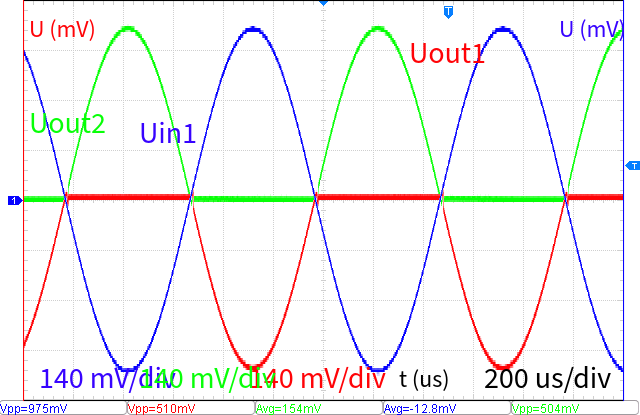
\includegraphics[width=0.8\textwidth]{lab/output1.png}
    \caption{Invertující zesilovač, nesym. napájení -- časový průběh správně zesíleného signálu.}
    \label{fig:lab/output1.png}
\end{figure}

\begin{figure}[h!]
    \centering
    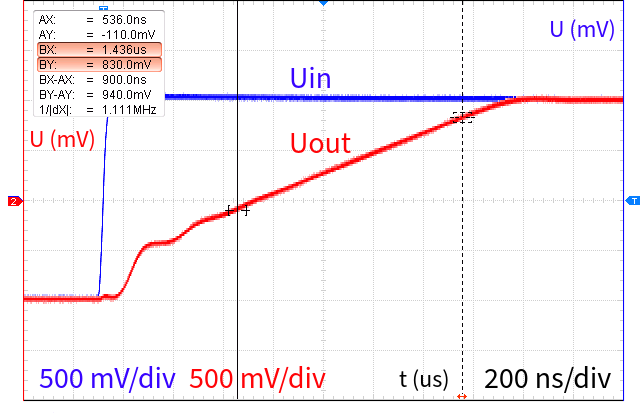
\includegraphics[width=0.9\textwidth]{lab/output2.png}
    \caption{Invertující zesilovač, nesym. napájení -- časový průběh správně zesíleného signálu, měřeno přímo na výstupu OZ, tedy s DC složkou.}
    \label{fig:lab-output2-png}
\end{figure}

\begin{figure}[h!]
    \centering
    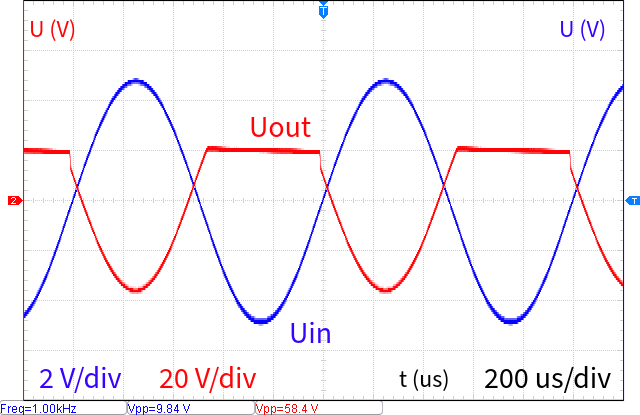
\includegraphics[width=0.9\textwidth]{lab/output3.png}
    \caption{Imvertující zesilovač, nesym. napájení -- změna poměru odporového děliče (\(R_4=\qty{100}{\kilo\ohm}\)) způsobila dosažení saturace.}
    \label{fig:lab-output3-png}
\end{figure}

\begin{figure}[h!]
    \centering
    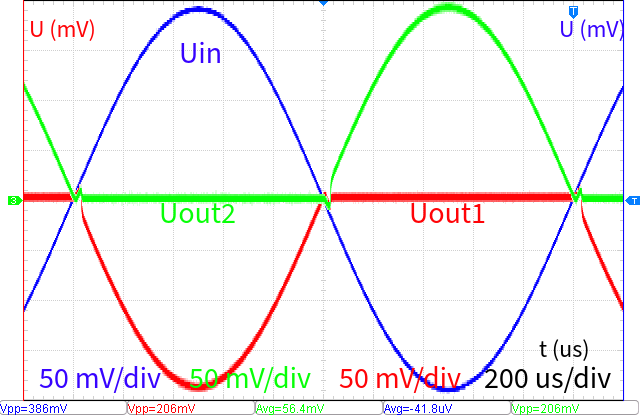
\includegraphics[width=0.9\textwidth]{lab/output4.png}
    \caption{Diferenční zesilovač -- dva vstupní signály se vzájemně odečtou a na výstupu invertují.}
    \label{fig:lab-output4-png}
\end{figure}


\begin{figure}[h!]
    \centering
    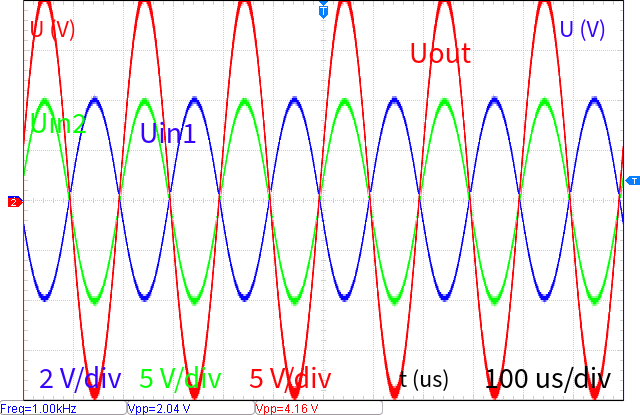
\includegraphics[width=0.9\textwidth]{lab/output5.png}
    \caption{Diferenční zesilovač -- dva opačné signály se opět odečtou, výsledkem je signál s dvojnásobnou amlitudou.}
    \label{fig:lab-output5-png}
\end{figure}

\begin{figure}[h!]
    \centering
    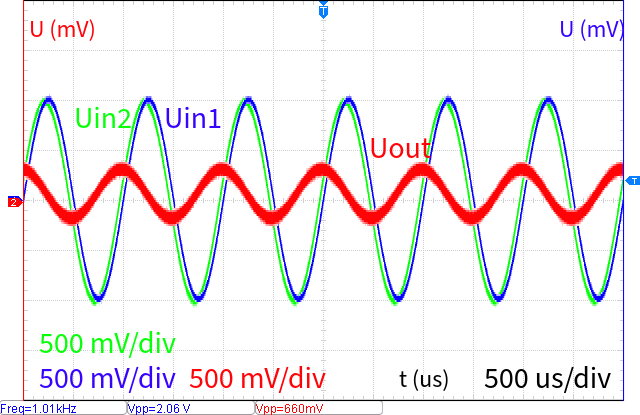
\includegraphics[width=0.9\textwidth]{lab/output6.png}
    \caption{Diferenční zesilovač -- odečtení dvou téměř shodných signálů, výsledný signál má mnohem nižší amplitudu.}
    \label{fig:lab-output6-png}
\end{figure}

\begin{figure}[h!]
    \centering
    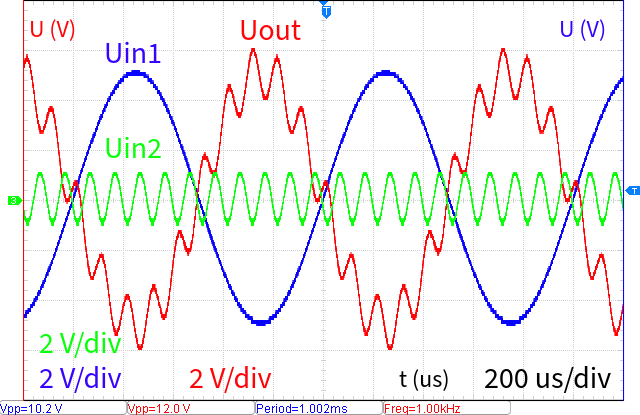
\includegraphics[width=0.9\textwidth]{lab/output7.png}
    \caption{Sumační zesilovač -- dva různé signály se na výstupu sečtou a následně invertují.}
    \label{fig:lab-output7-png}
\end{figure}

\begin{figure}[h!]
    \centering
    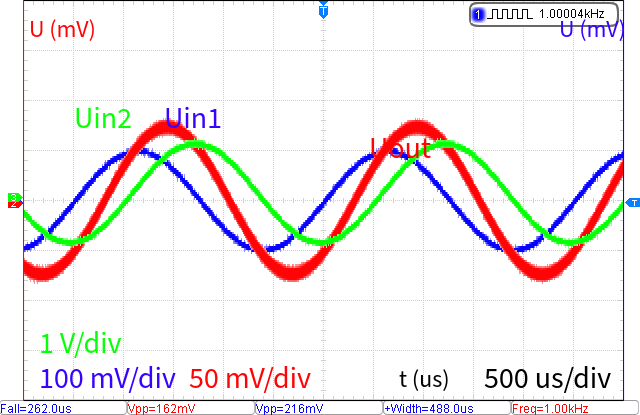
\includegraphics[width=0.9\textwidth]{lab/output8.png}
    \caption{Sumační zesilovač -- sečtení signálu s nulovým signálem vede k invertovanému původnímu signálu.}
    \label{fig:lab-output8-png}
\end{figure}



\begin{table}[h!]
    \centering
    \def\arraystretch{1.4}`'
    \caption{Stejnosměrný prac. bod, porovnání.}
    \begin{tabular}{|c|c|c|c|c|c|c|c|}
        \hline
            Č. uzlu & 1 & 2 & 3 & 4 & 5 &  6 &  7 \\
        \hline
            Výpočet & 15 & 7,5 & 7,5 & 7,5 & 7,5 &  0 &  0 \\
            Simulace & 15 & 7,499 & 7,499 & 7,499 & 7,499 &  0 &  0 \\
            Měření & 15,27 & 7,62 & 7,64 & 7,64 & 7,64 &  20m &  0 \\
        \hline
    \end{tabular}
    \label{tab:dc-bod}
\end{table}